\section*{Exercice 189 -- Correcteur proportionnel}
\setcounter{exo}{0}
%CCS MP 2010

\begin{obj}
Cette étude a pour objectif de synthétiser les paramètres des correcteurs à implanter afin d’éviter le
renversement d’un tube lors de sa mise en place dans le plateau. Dans cette partie, seule la synthèse du
correcteur dédié à la commande de l’actionneur $\left[M_2\right]$ associé à l’axe 2 est abordée.
\end{obj}

\begin{center}
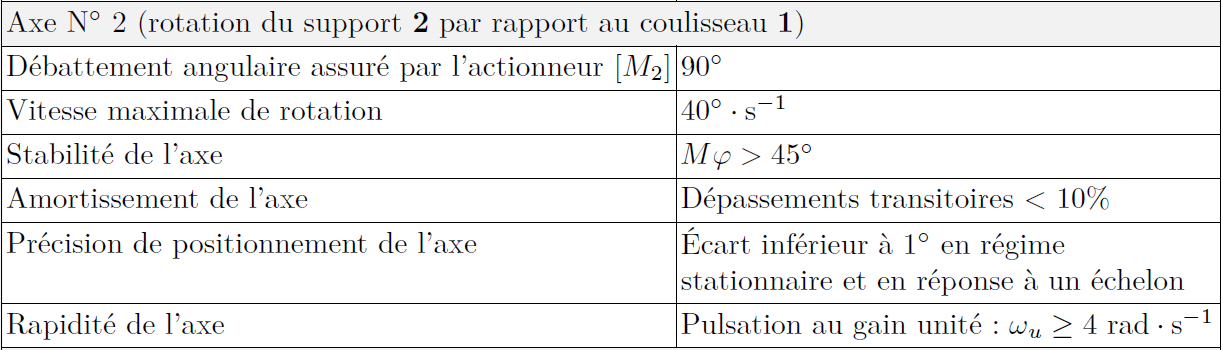
\includegraphics[width=\linewidth]{994_03}
\end{center}


Le correcteur à action proportionnelle est défini par la fonction de transfert suivante : $C(p) = K$.
On prendra comme Fonction de Transfert de la commande d’axe, la fonction $G(p) = \dfrac{K_2}{p\left(1+\tau p\right)}$ et comme architecture de commande le schéma bloc à retour unitaire de la figure suivante.

\begin{center}
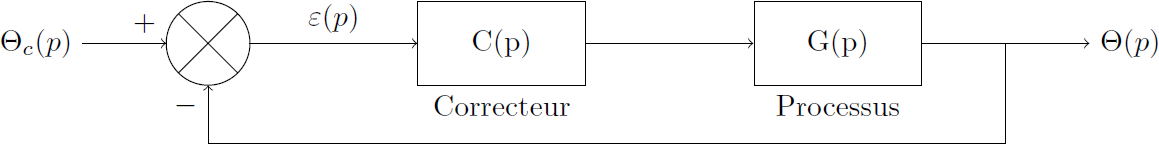
\includegraphics[width=\linewidth]{994_01}
\end{center}

On fournit le diagramme de Bode de la fonction de transfert $G(p)$.


\begin{center}
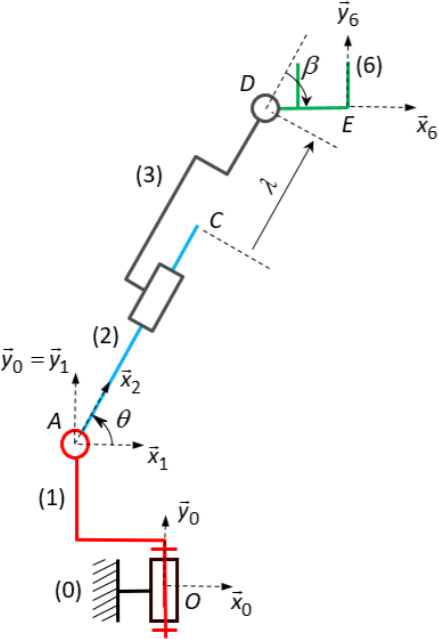
\includegraphics[width=\linewidth]{994_02}
\end{center}


\subparagraph{}
\textit{Justifier, à partir de ce diagramme, que le système en boucle fermée est stable.}
\ifprof
\begin{corrige}
\end{corrige}
\else
\fi


\subparagraph{}
\textit{Déterminer la valeur de l’écart en régime stationnaire pour un échelon de consigne d’amplitude $\theta_0$.
Conclure quant au respect du cahier des charges.}
\ifprof
\begin{corrige}
\end{corrige}
\else
\fi

Afin de respecter le temps d’exécution, le cahier des charges impose que la pulsation au gain unité de la boucle
ouverte $\omega_u$ soit au moins égale à $\SI{4}{rad.s^{-1}}$.

\subparagraph{}
\textit{Déterminer la valeur minimale du gain $K$ du correcteur à action proportionnelle assurant la validation
du critère de performance en rapidité. En déduire la valeur de la marge de phase $M\varphi$ pour cette valeur de $K$.
Conclure quant au respect du cahier des charges.}
\ifprof
\begin{corrige}
\end{corrige}
\else
\fi

